% ------------------------------------------------------------------------------
% TYPO3 CMS 7.4 - What's New (English Version)
%
% @author	Michael Schams <schams.net>
% @license	Creative Commons BY-NC-SA 3.0
% @link		http://typo3.org/download/release-notes/whats-new/
% @language	English
% ------------------------------------------------------------------------------
% LTXE-CHAPTER-UID:		0dbe76ce-5948c314-454b95fd-543cb62c
% LTXE-CHAPTER-NAME:	Backend User Interface
% ------------------------------------------------------------------------------

\section{Administratorski interfejs}
\begin{frame}[fragile]
	\frametitle{Administratorski interfejs}

	\begin{center}\huge{Poglavlje 1:}\end{center}
	\begin{center}\huge{\color{typo3darkgrey}\textbf{Administratorski interfejs}}\end{center}

\end{frame}

% ------------------------------------------------------------------------------
% LTXE-SLIDE-START
% LTXE-SLIDE-UID:		c2e058bf-b60614cc-a322bf46-5c73d1ef
% LTXE-SLIDE-ORIGIN:	464d4ba6-dab07499-0cd5f168-552e9729 English
% LTXE-SLIDE-ORIGIN:	8080f469-3c5592f0-dc25ad87-894c2648 German
% LTXE-SLIDE-TITLE:		Feature: #48947 - Avatars for backend users
% LTXE-SLIDE-REFERENCE:	Feature-48947-AvatarsForBackendUsers.rst
% ------------------------------------------------------------------------------
\begin{frame}[fragile]
	\frametitle{Administratorski interfejs}
	\framesubtitle{Avatari za korisnike administratorskog interfejsa}

	Kako bi se poboljsalo korisnicko iskustvo u zajednickom editovanju sadrzaja, urednici sada mogu koristiti avatare. Ove male korisnicke slicice prikazuju se u gornjem baru, listi korisinika i na drugim mestima.

	\begin{figure}
		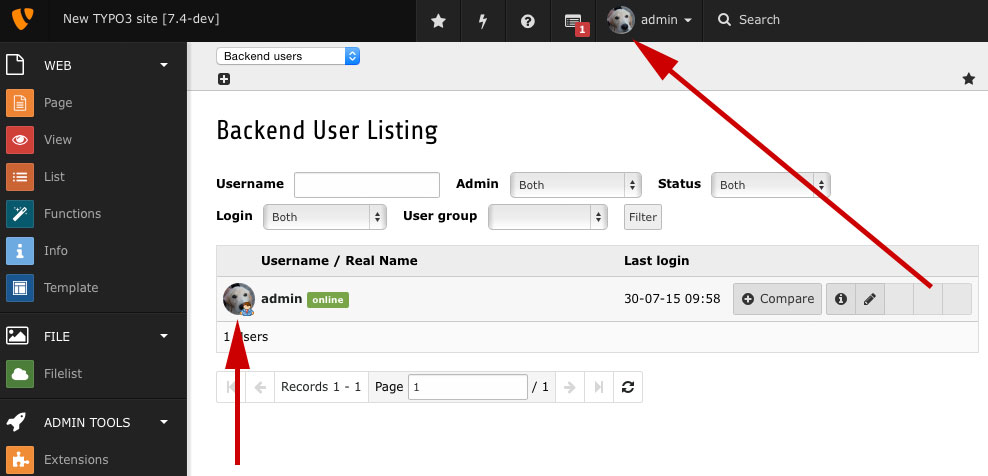
\includegraphics[width=0.9\linewidth]{BackendUserInterface/48947.jpg}
	\end{figure}

\end{frame}

% ------------------------------------------------------------------------------
% LTXE-SLIDE-START
% LTXE-SLIDE-UID:		69683faa-ce4f2210-6be207cf-0cf8879a
% LTXE-SLIDE-ORIGIN:	89f348c8-db045eff-5dfc4f42-da1a2cfa English
% LTXE-SLIDE-ORIGIN:	b0f7e15a-7cc72aaa-79738ec7-643c5cec German
% LTXE-SLIDE-TITLE:		Feature: #56133 - Replace file feature for fal file list
% LTXE-SLIDE-REFERENCE:	Feature-56133-ReplaceFileFeatureForFalFileList.rst
% ------------------------------------------------------------------------------
\begin{frame}[fragile]
	\frametitle{Administratorski interfejs}
	\framesubtitle{Zamena fajlova}

	Fajlovi u FAL rekord listi sada mogu biti \textbf{zamenjeni} (moga biti omogucen "extended view"). Ime fajla postojeceg fajla moze da se zadrzi ili promeni.

	\begin{figure}
		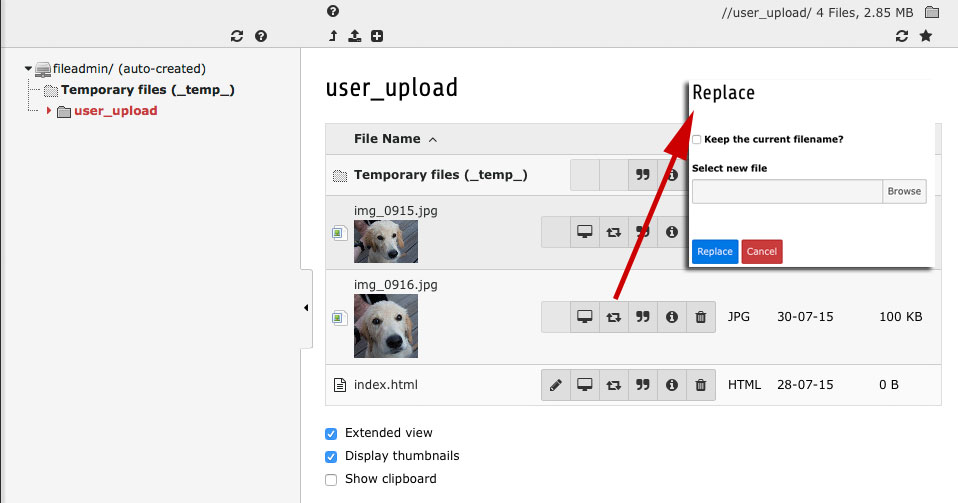
\includegraphics[width=0.75\linewidth]{BackendUserInterface/56133.jpg}
	\end{figure}

\end{frame}

% ------------------------------------------------------------------------------
% LTXE-SLIDE-START
% LTXE-SLIDE-UID:		6f419340-4a9cd2f6-947f12a1-29077b57
% LTXE-SLIDE-ORIGIN:	7e5987f7-9a91ea61-8564c721-0f8d5e4a English
% LTXE-SLIDE-ORIGIN:	613354cc-9475feef-bec620c5-31170549 German
% LTXE-SLIDE-TITLE:		Feature: #67574 - Display online status in backend user list
% LTXE-SLIDE-REFERENCE:	Feature-67574-DisplayOnlineStatusInBackendUserList.rst
% ------------------------------------------------------------------------------
\begin{frame}[fragile]
	\frametitle{Administratorski interfejs}
	\framesubtitle{Online status za korisnike administratorskog interfejsa}

	Online status za korisnike administratorskog interfejsa moze se videti u "Backend Users" modulu.

	\begin{figure}
		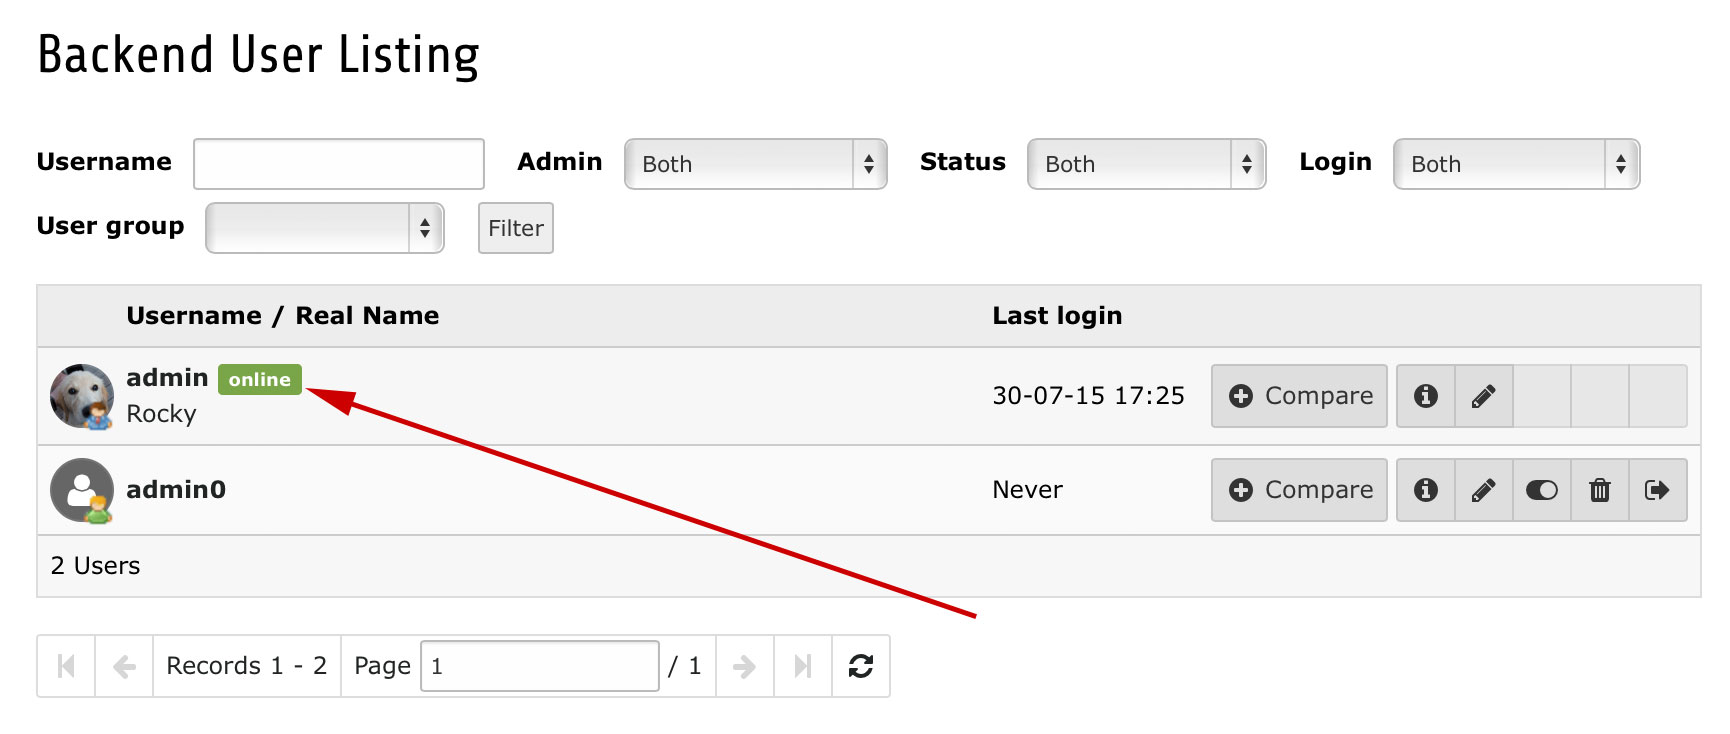
\includegraphics[width=0.9\linewidth]{BackendUserInterface/67574.jpg}
	\end{figure}

\end{frame}

% ------------------------------------------------------------------------------
% LTXE-SLIDE-START
% LTXE-SLIDE-UID:		7ee839b9-ad8f08bd-0e243059-a2a2b711
% LTXE-SLIDE-ORIGIN:	0154fc51-74683590-ebbe8559-ce6a0d57 English
% LTXE-SLIDE-ORIGIN:	00c93fe2-9d128591-20b71814-13556f43 German
% LTXE-SLIDE-TITLE:		FormEngine: Drop "Show secondary options"
% LTXE-SLIDE-REFERENCE:	https://forge.typo3.org/issues/67753
% ------------------------------------------------------------------------------
\begin{frame}[fragile]
	\frametitle{Administratorski interfejs}
	\framesubtitle{Sekundarne opcije uklonjene}

	Cekboks "Show secondary options (palettes)", TScong opcija strane \texttt{options.enableShowPalettes} i TCA podesavanje su uklonjeni. Palete su uvek vidljive i sada se vise ne mogu sakriti.

	\begin{figure}
		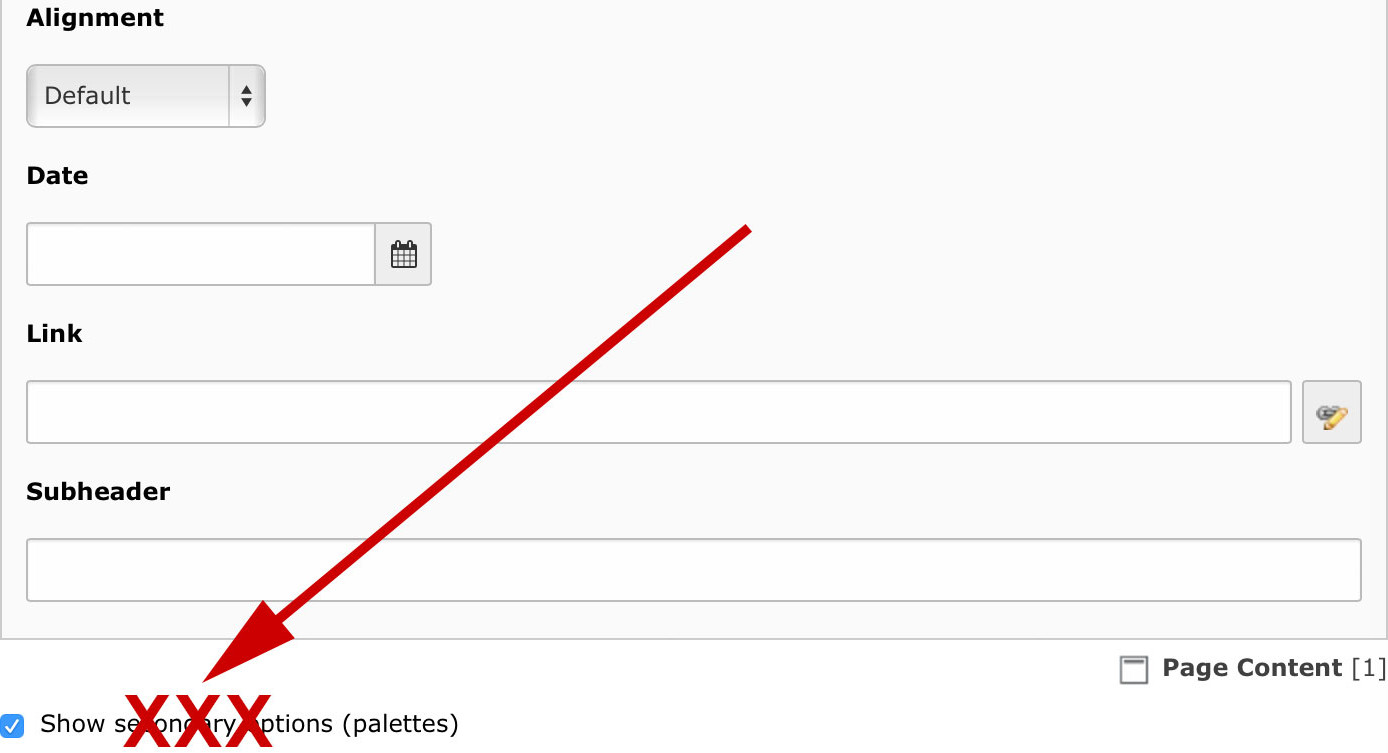
\includegraphics[width=0.7\linewidth]{BackendUserInterface/67753.jpg}
	\end{figure}

\end{frame}

% ------------------------------------------------------------------------------
% LTXE-SLIDE-START
% LTXE-SLIDE-UID:		9f906832-7b28a31b-3289cc41-4fbd3758
% LTXE-SLIDE-ORIGIN:	f9b24e36-28e8872c-41297de9-52467554 English
% LTXE-SLIDE-ORIGIN:	bab4e93d-0a6d4612-41b2f67e-47c37ff7 German
% LTXE-SLIDE-TITLE:		Feature: #67578 - Add description-field for backend-users
% LTXE-SLIDE-REFERENCE:	Feature-67578-AddDescriptionFieldForBeUsers.rst
% ------------------------------------------------------------------------------
\begin{frame}[fragile]
	\frametitle{Administratorski interfejs}
	\framesubtitle{Opis za korisnike administratorskog interfejsa}

	Novo polje "Description" dodato je rekordima koji se ticu korisnika administratorskog interfejsa.

	\begin{figure}
		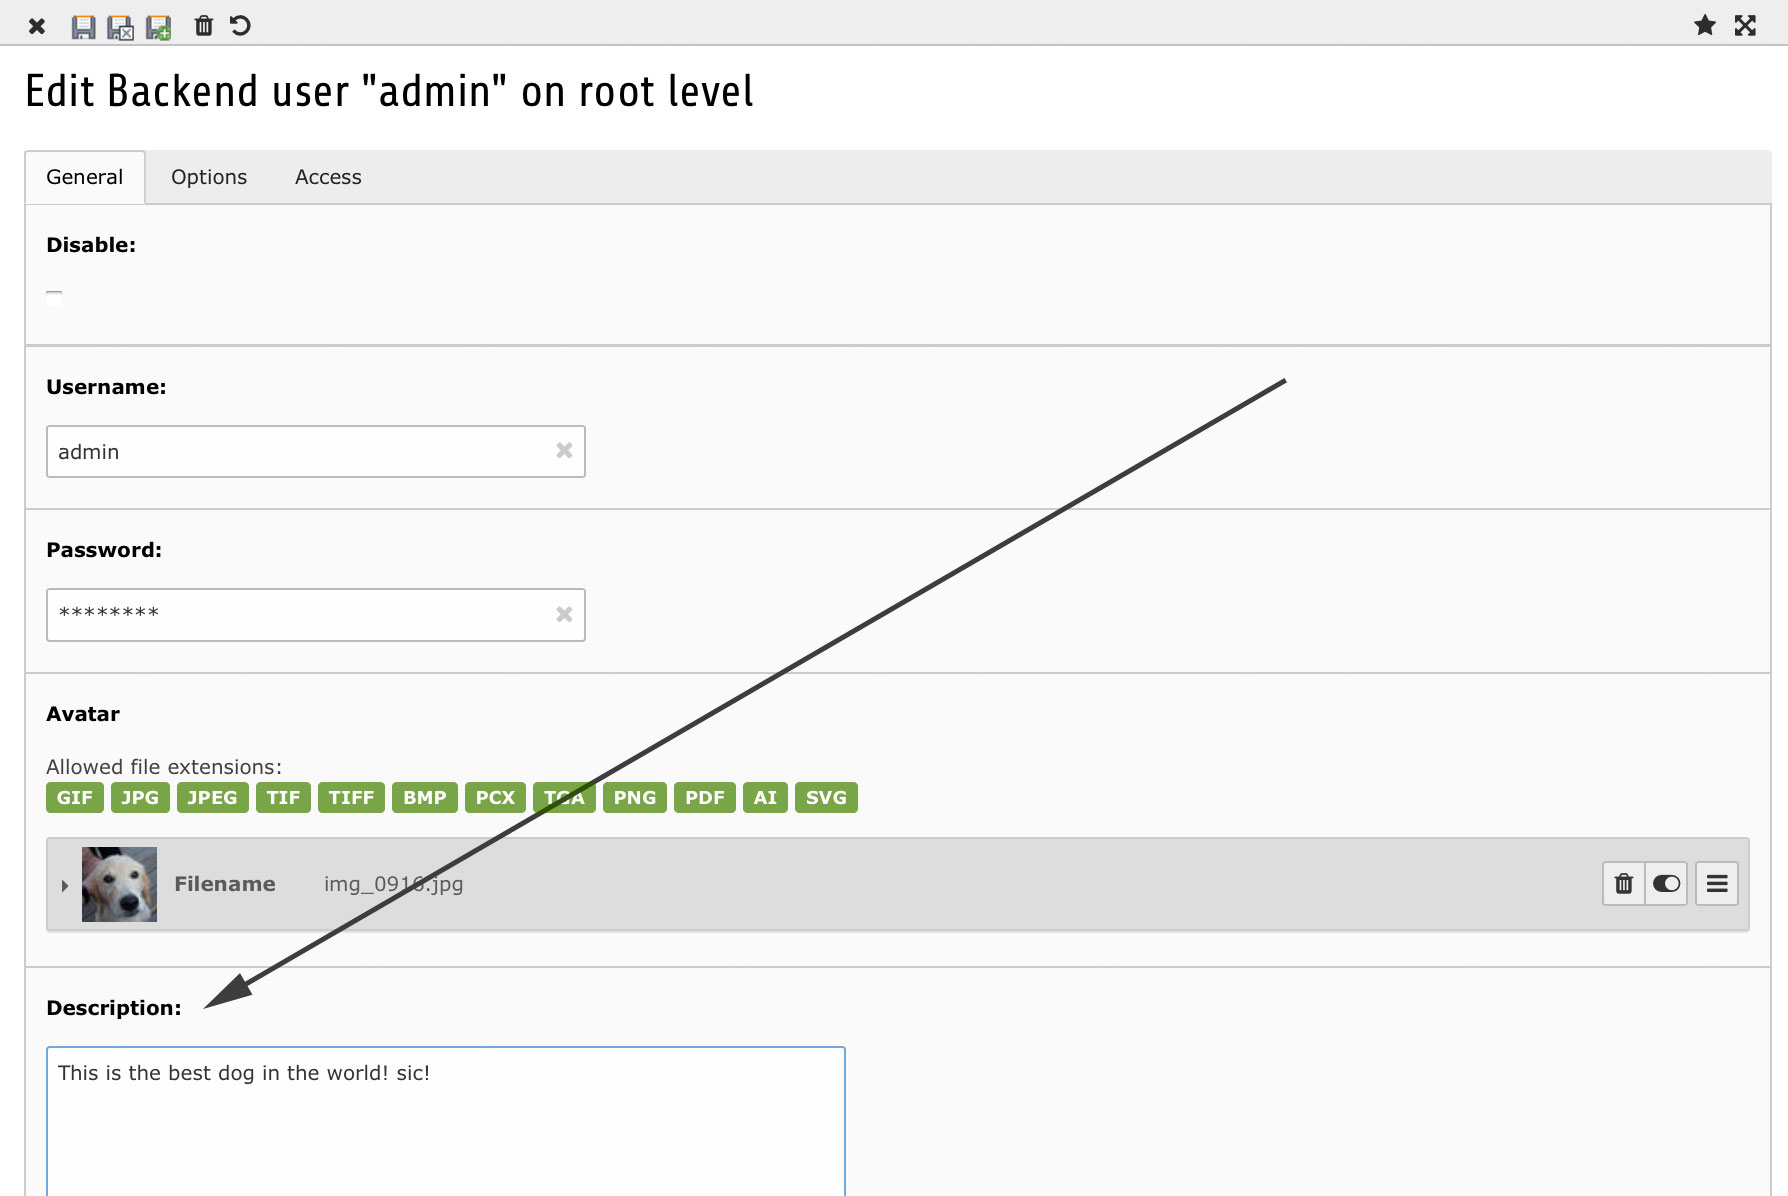
\includegraphics[width=0.7\linewidth]{BackendUserInterface/67578.jpg}
	\end{figure}

\end{frame}

% ------------------------------------------------------------------------------
% LTXE-SLIDE-START
% LTXE-SLIDE-UID:		8125e791-ca227a79-71f6252d-a2b0c5d6
% LTXE-SLIDE-ORIGIN:	83db5442-fa2edfcc-925dd5b6-4afe26f5 English
% LTXE-SLIDE-ORIGIN:	649bd9ee-240381c8-950424ea-f032775b German
% LTXE-SLIDE-TITLE:		Feature: #67603 - Introduce TCA > ctrl > descriptionColumn
% LTXE-SLIDE-REFERENCE:	Feature-67603-IntroduceTcaDescriptionColumn.rst
% ------------------------------------------------------------------------------
\begin{frame}[fragile]
	\frametitle{Administratorski interfejs}
	\framesubtitle{Opis za kolone tabela}

	Konfiguracijom kolona (najcesce \texttt{opis}) u podesavanjima TCA \texttt{[’TCA’][’ctrl’][’descriptionColumn’]}, moze se prikazati opis (poboljsava upotrebljivost za urednike i administratore).

	\begin{figure}
		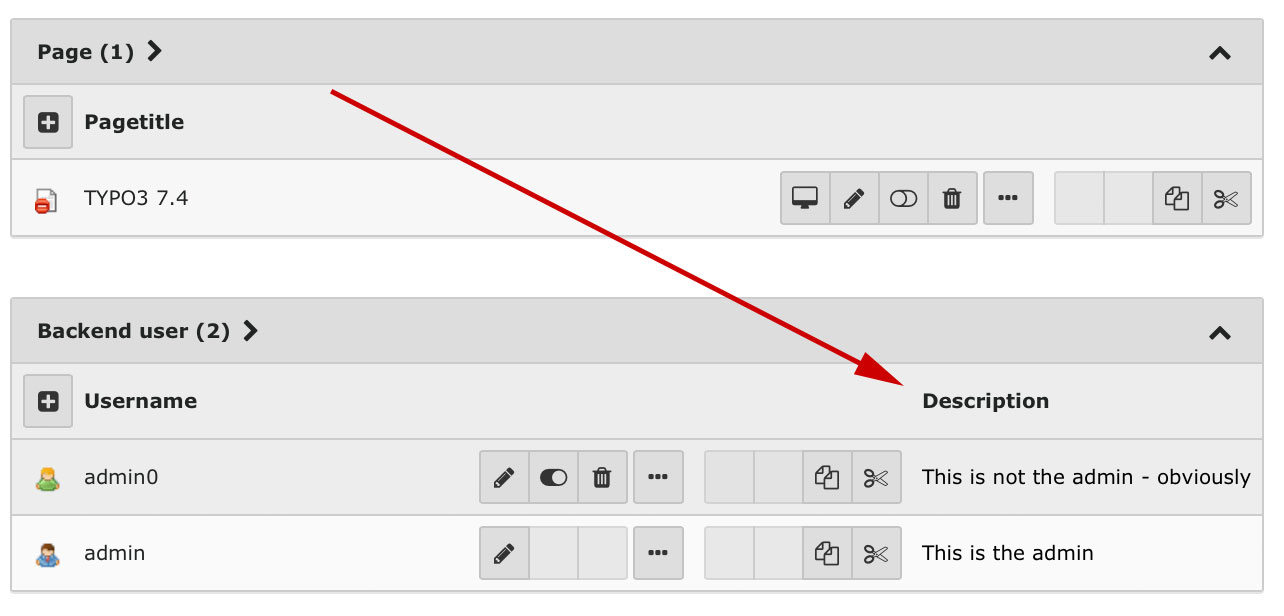
\includegraphics[width=0.7\linewidth]{BackendUserInterface/67603.jpg}
	\end{figure}

\end{frame}

% ------------------------------------------------------------------------------
% LTXE-SLIDE-START
% LTXE-SLIDE-UID:		57b6b17e-87fe658a-8b0b0911-9d3c2375
% LTXE-SLIDE-ORIGIN:	7c5400a9-c4b667f3-1a0c046a-9dd3b6a9 English
% LTXE-SLIDE-ORIGIN:	2eeaec46-1929743b-8e6f9285-13d20d3c German
% LTXE-SLIDE-TITLE:		Feature: #59570 - Add description-field for filemounts
% LTXE-SLIDE-REFERENCE:	Feature-59570-AddDescriptionFieldForFilemounts.rst
% ------------------------------------------------------------------------------
\begin{frame}[fragile]
	\frametitle{Administratorski interfejs}
	\framesubtitle{Opis za skladiste fajlova (filemounts)}

	Novo polje "Description" dodato je rekordima koji se ticu skladista fajlova. Polje omogucava administratorima da dodaju kratki opis o tome za sta se odredjeno skladiste fajlova koristi, koje fajlove sadrzi itd.

	\begin{figure}
		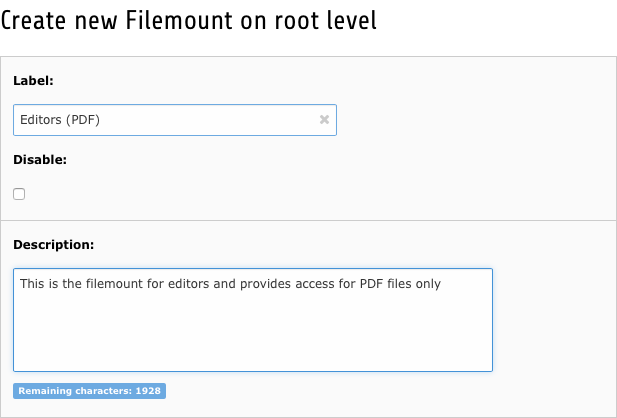
\includegraphics[width=0.55\linewidth]{BackendUserInterface/59570.png}
	\end{figure}

\end{frame}

% ------------------------------------------------------------------------------
% LTXE-SLIDE-START
% LTXE-SLIDE-UID:		69ab6189-7ff25725-b4469d37-256a5af4
% LTXE-SLIDE-ORIGIN:	d00f63c4-05272792-21a0a301-4d6a726c English
% LTXE-SLIDE-ORIGIN:	879b1dda-9167d830-373f7457-0391ebee German
% LTXE-SLIDE-TITLE:		Feature: #68197 - Show a dialog for existing files on upload
% LTXE-SLIDE-REFERENCE:	Feature-68197-ShowADialogForExistingFilesOnUpload.rst
% ------------------------------------------------------------------------------
\begin{frame}[fragile]
	\frametitle{Administratorski interfejs}
	\framesubtitle{Upozorenje za postojece fajlove prilikom dodavanja novih}

	Ukoliko ce novi fajl pregaziti vec postojeci fajl, prikazuje se upozorenje koje pita korisnika da izabere akciju (npr. zameni, preimenuj ili preskoci).

	\begin{figure}
		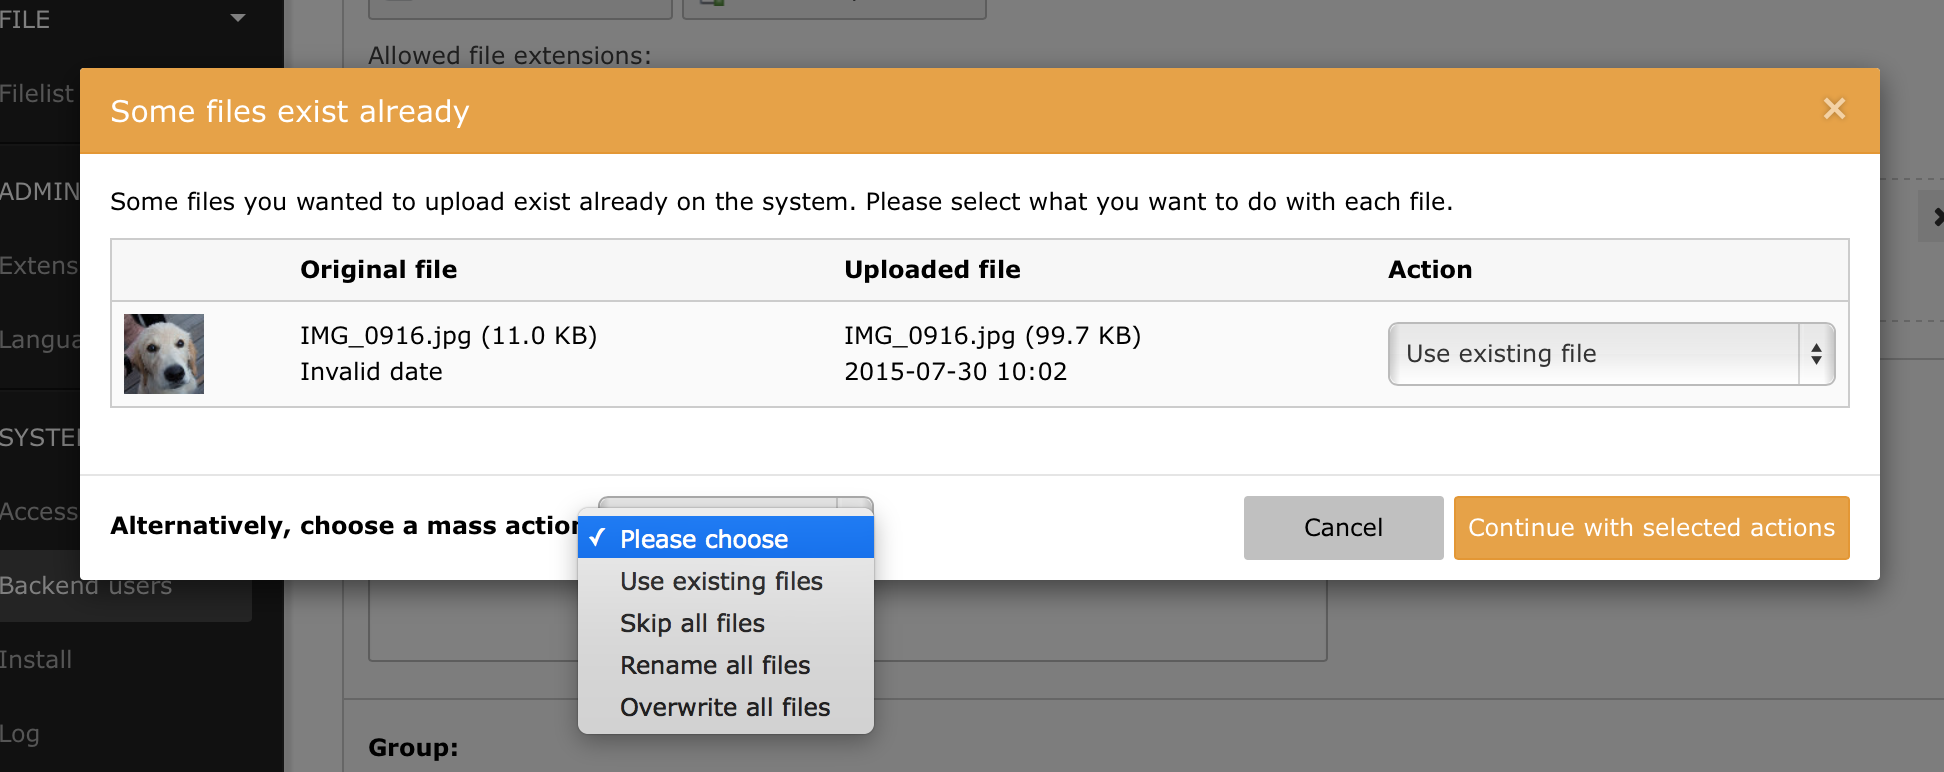
\includegraphics[width=0.9\linewidth]{BackendUserInterface/68197.png}
	\end{figure}

\end{frame}


% ------------------------------------------------------------------------------
% LTXE-SLIDE-START
% LTXE-SLIDE-UID:		fa2287f6-d3ce94f8-542f9687-b2b2c245
% LTXE-SLIDE-ORIGIN:	31d7dd8e-a3c71be4-309850ab-45a7db72 English
% LTXE-SLIDE-ORIGIN:	f4baa7b8-2237ad1d-5c4be365-a845f207 German
% LTXE-SLIDE-TITLE:		Feature: #68218 - Lock edit for tt_content
% LTXE-SLIDE-REFERENCE:	Feature-68218-LockEditForTt_content.rst
% ------------------------------------------------------------------------------
\begin{frame}[fragile]
	\frametitle{Administratorski interfejs}
	\framesubtitle{Restrikcije u editovanju elemenata sadrzaja}

	Elementi sadrzaja sada mogu biti ograniceni da mogu trpeti izmene samo od administratora (slicno funkciji za strane "Restrict editing by non-Admins").

	\begin{figure}
		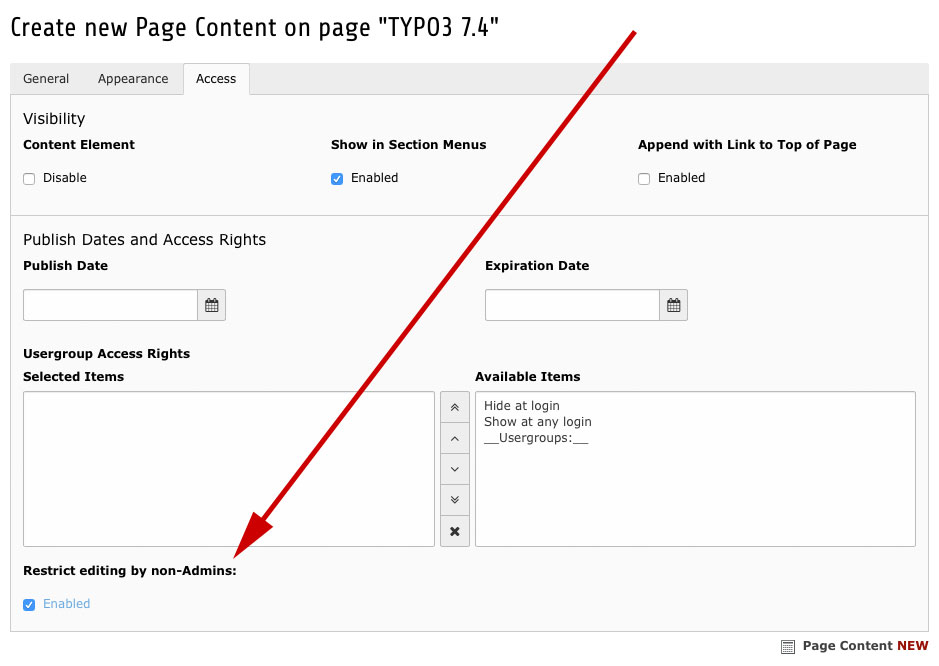
\includegraphics[width=0.6\linewidth]{BackendUserInterface/68218.jpg}
	\end{figure}

\end{frame}

% ------------------------------------------------------------------------------
% LTXE-SLIDE-START
% LTXE-SLIDE-UID:		5b8c6ff2-ff16c2bc-f1b3280a-1395e080
% LTXE-SLIDE-ORIGIN:	4e60055a-266e3e24-7baa1613-1226575e English
% LTXE-SLIDE-ORIGIN:	bc83e40f-9b7bac03-ea5f07c4-be27eb56 German
% LTXE-SLIDE-TITLE:		Feature: #68315 - Include pageTSconfig file (1)
% LTXE-SLIDE-REFERENCE:	Feature-68315-IncludeAPageTSconfigFileInPagePropertiesLikeTSStaticTemplates.rst
% ------------------------------------------------------------------------------
\begin{frame}[fragile]
	\frametitle{Administratorski interfejs}
	\framesubtitle{Ukljucivanje Static TSconfig fajlova (1)}

	U dodatnim podesavanjima strane postoji opcija za ukljucivanje TSconfig fajla na strani (isti nacin na koji se ukljucuje TypoScript).

	\begin{figure}
		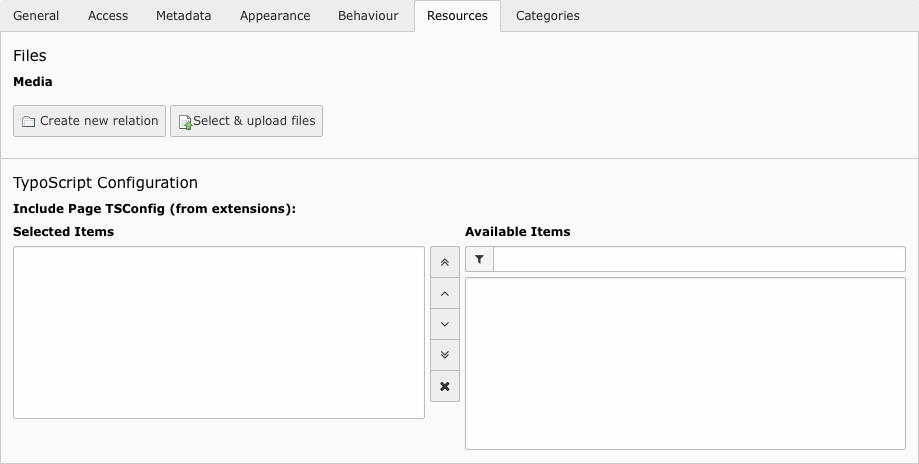
\includegraphics[width=0.8\linewidth]{BackendUserInterface/68315.png}
	\end{figure}

\end{frame}

% ------------------------------------------------------------------------------
% LTXE-SLIDE-START
% LTXE-SLIDE-UID:		84459747-f8bd3560-d7a7b5ab-29722bce
% LTXE-SLIDE-ORIGIN:	4f5cb411-3ea84dfd-84edb16d-433b9fc5 English
% LTXE-SLIDE-ORIGIN:	9b7bac03-ea5f07c4-be27eb56-ac03e27e German
% LTXE-SLIDE-TITLE:		Feature: #68315 - Include pageTSconfig file (2)
% LTXE-SLIDE-REFERENCE:	Feature-68315-IncludeAPageTSconfigFileInPagePropertiesLikeTSStaticTemplates.rst
% ------------------------------------------------------------------------------
\begin{frame}[fragile]
	\frametitle{Administratorski interfejs}
	\framesubtitle{Ukljucivanje Static TSconfig fajlova (2)}

	% decrease font size for code listing
	\lstset{basicstyle=\tiny\ttfamily}

	Sledeci metod registruje TSconfig fajl strane:

	\begin{lstlisting}
		\TYPO3\CMS\Core\Utility\ExtensionManagementUtility::registerPageTSConfigFile(
		  'extension_name',
		  'Configuration/PageTS/myPageTSconfigFile.txt',
		  'My special configuration'
		);
	\end{lstlisting}

\end{frame}

% ------------------------------------------------------------------------------
% LTXE-SLIDE-START
% LTXE-SLIDE-UID:		be833e1e-d4ecebee-18c09459-a877dd54
% LTXE-SLIDE-ORIGIN:	c00b2bfd-2c1b02b0-a7ef9cd0-62f147d2 English
% LTXE-SLIDE-ORIGIN:	f8d888b1-b93dcf4a-e20b976e-9a5c277e German
% LTXE-SLIDE-TITLE:		Feature: #68395 - Allow real copies of content elements into foreign languages
% LTXE-SLIDE-REFERENCE:	Feature-68395-AllowRealCopiesOfContentElementsIntoForeignLanguages.rst
% ------------------------------------------------------------------------------
\begin{frame}[fragile]
	\frametitle{Administratorski interfejs}
	\framesubtitle{Stvarne kopije elemenata sadrzaja}

	Dodato je novo dugme svakoj koloni na "Page" modulu koje dozvoljava stvarne kopije elemenata sadrzaja na drugim jezicima (ne samo reference).

	\begin{figure}
		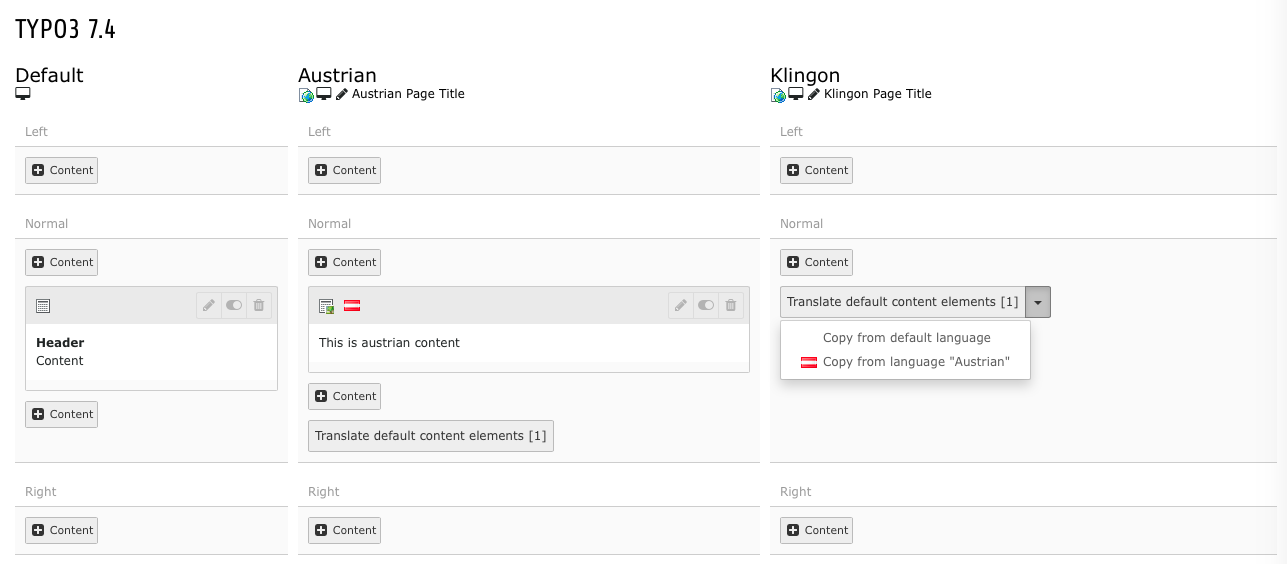
\includegraphics[width=0.9\linewidth]{BackendUserInterface/68395.png}
	\end{figure}

\end{frame}


